%!TEX root = syntheyes15.tex

\section{Rendering photo-realistic training images}

We briefly describe how we use image-based lighting \cite{debevec2002image} to model a wide range of realistic lighting conditions, and finally discuss the details of our rendering setup.

\begin{figure}
    \centering
    \begin{subfigure}[t]{0.48\columnwidth}
        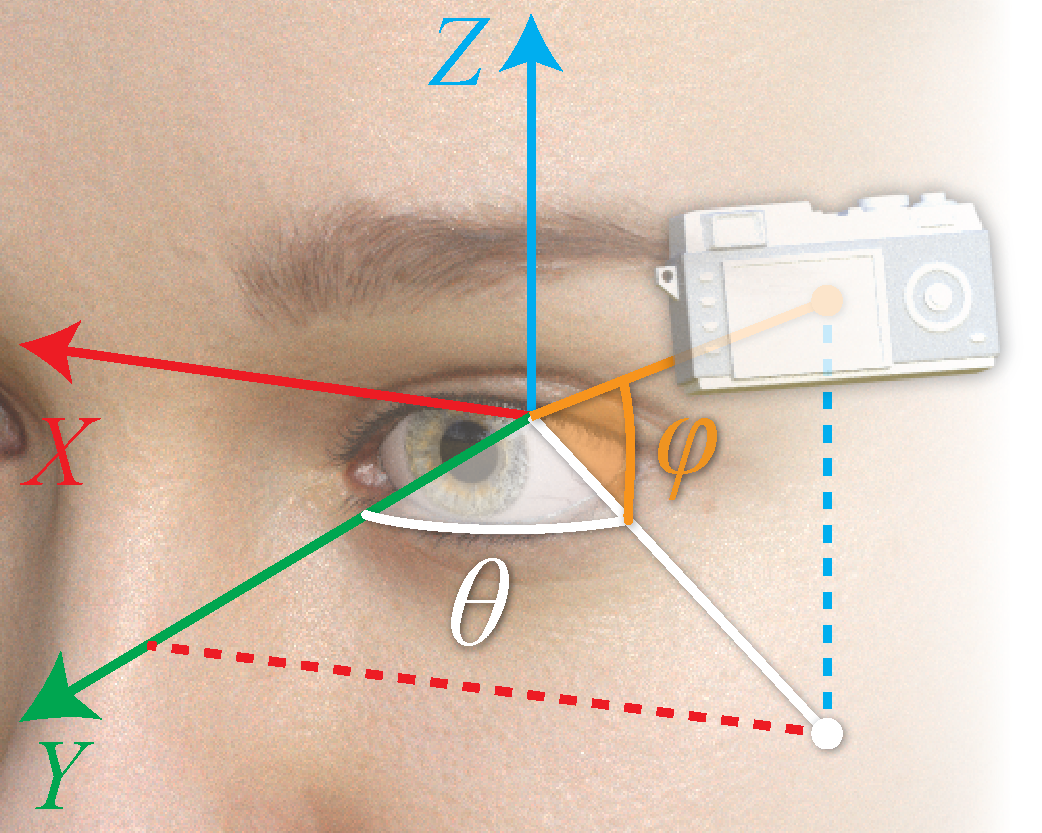
\includegraphics[width=\textwidth]{camera_position}
        \caption{The camera is positioned using spherical coordinates}
        \label{fig:cam_pos_spher_coords}
    \end{subfigure}
    \hfill
    \begin{subfigure}[t]{0.48\columnwidth}
        \includegraphics[width=\textwidth]{camera_pos_sample_renders_7x7}
        \caption{Example renderings from one camera position}
        \label{fig:cam_pos_example_renders}
    \end{subfigure}
    \caption{\ref{fig:cam_pos_spher_coords} shows how we position the camera to simulate changes in head pose. At each camera position, we render many eye images (\ref{fig:cam_pos_example_renders}) by posing the eyeball model.}
\end{figure}

\subsection{Lighting}

\begin{figure}
    \includegraphics[width=0.24\columnwidth]{fig_env_1} \hfill
    \includegraphics[width=0.24\columnwidth]{fig_env_2} \hfill
    \includegraphics[width=0.24\columnwidth]{fig_env_3} \hfill
    \includegraphics[width=0.24\columnwidth]{fig_env_4}
    \caption{Appearance variation from lighting is modelled with poseable high-dynamic-range environment maps \cite{debevec2002image}.}
    \label{fig:participants}
\end{figure}

\subsection{Computational setup}

We can rapidly generate diverse datasets much faster than manual collection and annotation.